\section{Slurm Workload Manager}
\label{sec:slurm}

Slurm Workload Manager is an open-source cluster management and job scheduling system for Linux-based high-performance computing environments \cite{yoo2003slurm, slurm2024docs}. It is widely deployed in research and production HPC clusters, including large systems represented in the TOP500 list \cite{schedmd2024slurm}. This project uses Slurm as the target operational domain because it exposes a rich command surface for monitoring, diagnosis, submission, accounting, and controlled cluster administration.

\subsection{Architecture Overview}

Slurm follows a controller-and-worker architecture. The central controller maintains cluster state and scheduling decisions, while node-level daemons execute and monitor workloads.

The \textbf{slurmctld} daemon is the central controller. It tracks nodes, partitions, jobs, reservations, and resource allocations. It accepts job submissions, evaluates pending work, applies scheduling policy, and dispatches jobs to available compute resources. In production clusters, a backup controller can be configured for high availability.

\begin{figure}[H]
    \centering
    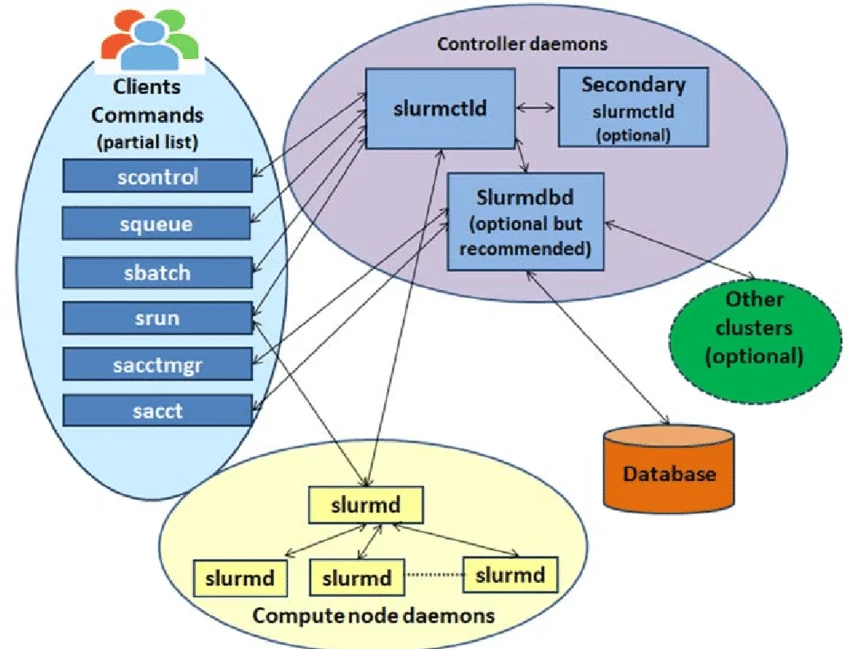
\includegraphics[width=0.8\textwidth]{images/slurm_resource_management.png}
    \caption{Slurm master-worker architecture. Client commands (\texttt{sbatch}, \texttt{srun}, \texttt{squeue}) submit requests to the central \texttt{slurmctld} controller daemon, which schedules work and dispatches it to per-node \texttt{slurmd} daemons on compute nodes. An optional \texttt{slurmdbd} accounting daemon records job history in a persistent database for later retrieval via \texttt{sacct}. A secondary \texttt{slurmctld} can be configured for high availability, and the controller may communicate with external clusters for multi-cluster management~\cite{abhishek2022dynamic}.}
    \label{fig:slurm-architecture}
\end{figure}

The \textbf{slurmd} daemon runs on each compute node. It launches job steps, monitors local execution, reports node state to the controller, and handles job control signals. This makes the compute node visible to the scheduler while preserving local execution responsibility.

The \textbf{slurmdbd} daemon provides the accounting service when enabled. It stores job history, user associations, account usage, fair-share information, and reporting data in a database. These records are important for administrative workflows, quota analysis, and historical job diagnosis.

\subsection{Core Operational Objects}

Slurm operations are built around several core objects:

\textbf{Nodes} are compute servers with resources such as CPUs, memory, GPUs, and generic resources. Node state matters operationally: an idle node can accept work, an allocated node is running jobs, a drained node is intentionally unavailable for new work, and a down node is unavailable because of failure or administrative action.

\textbf{Partitions} are logical groups of nodes. They behave like queues and encode access rules, limits, default policies, and intended usage patterns. Users often need to know which partition matches a job's resource requirements and policy constraints.

\textbf{Jobs} are resource allocation requests. A job includes requested resources, time limits, partition, account or QoS settings, script or command, and optional dependencies. Jobs move through states such as pending, running, completed, failed, cancelled, held, or suspended.

\textbf{Steps} are execution units inside an allocated job. A job may contain one or more steps, and step-level inspection is useful for understanding running work, CPU usage, memory behavior, and launched parallel tasks.

\textbf{Accounts, QoS, and reservations} represent policy and access constraints. They affect who can submit work, how resources are charged, which jobs receive priority, and when nodes are reserved for maintenance or special workloads.

These objects are accessed through a broad command surface. Read-only commands such as \texttt{sinfo}, \texttt{squeue}, \texttt{sacct}, and \texttt{scontrol show} inspect partitions, jobs, accounting records, nodes, reservations, and configuration state. Other commands, including \texttt{sbatch}, \texttt{srun}, \texttt{salloc}, \texttt{scancel}, selected \texttt{scontrol} operations, and \texttt{sacctmgr}, can submit work or modify jobs, nodes, reservations, accounts, and QoS policies. The same command family may contain both safe inspection operations and high-impact administrative operations; for example, \texttt{scontrol show job} is read-only, while \texttt{scontrol update} can change job or node state. This distinction is central to the Observer/Operator design used later in the thesis.

\subsection{Why Slurm Is Difficult to Use Through Natural Language}

Slurm's command-line interface is expressive, but that expressiveness creates usability and safety challenges. Users must know command names, flags, output formats, state meanings, pending reasons, account/QoS concepts, and site-specific policy conventions. Many operations are also state-dependent: cancelling a running job, releasing a held job, or updating a reservation only makes sense when the referenced object exists and is in an appropriate state.

These properties make Slurm a useful but demanding domain for a natural-language agent. The agent must map user intent to the correct command surface, obtain live cluster facts when needed, distinguish documentation questions from operational questions, and require explicit confirmation before state-changing actions are executed.
